\chapter{Konzeption}
\label{Konzeption}
In diesem Kapitel wird die geplante Architektur des verteilten Systems beschrieben. \\
Generell wird die Kommunikation nachrichtenbasiert umgesetzt. Dies bedeutet, dass die Komponenten des verteilten Systems kommunizieren, indem sie sich Nachrichten übermitteln können. Die Steuerung der Kommunikation wird primär von den als Master 
(siehe \ref{glossar}) ausgewählten Komponenten umgesetzt. Als Provider wird ein angepasster Webserver eingesetzt, die Verbindung der einzelnen Komponenten zueinander geschieht über WebSockets. Der Webserver basiert auf dem Javascript-Framework Node.js. \\


\section{Brute Force-Algorithmus}
\label{ideeBruteForce}
Grundlegend ist das Ziel des Projektes das Entschlüsseln eines vorgegebenen Passwortes. Das zu entschlüsselnde Passwort wird vor der Berechnung vom Benutzer eingetragen. Das eingetragene Passwort wird dann durch eine Hashfunktion geleitet. Der entstandene Hash wird gespeichert und dient als Zielbedingung der folgenden Berechnung. \\
Nun beginnt der eigentliche Angriff. Zu Beginn wird eine sogenannte \enquote{Dictionary-Attack} vorgenommen. Dies bedeutet, dass ein Wörterbuch mit häufig genutzten Passwörtern als Basis des Angriffs genutzt wird. Durch die vorangestellte Attacke auf Basis von häufig benutzten Passwörtern wird die Wahrscheinlichkeit des effizienten Entschlüsseln des gesuchten Passworts erhöht. \\
Bleibt die Dictionary-Attack erfolglos, werden alle möglichen Zeichenkombinationen untersucht. \\
Die erste Idee war es, dass der steuernde Rechner alle möglichen Passwörter in einem Array ablegen wird. Das Muster der möglichen Passwörter sollte wie folgt aufgebaut werden: 

\texttt{Muster der zu berechnenden Passwörter:}
\begin{lstlisting}[basicstyle=\ttfamily,numbers=left,numberstyle=\footnotesize\ttfamily,backgroundcolor=\color{sourcegray}]
	Array passwordsUPPER = 
		[A*****,
	 	B*****,
	 	C*****,
	 	D*****,
	 	...
	]
	
	
	Array passwordsLOWER = 
		[a*****,
	 	b*****,
	 	c*****,
	 	d*****,
		...
	]
	
	

	Array passwordsNUM = 
		[1*****,
	 	2*****,
	 	3*****,
	 	4*****,
		...
	]
\end{lstlisting}

Die exemplarische Darstellung soll die geplante Aufteilung verdeutlichen. Die hier dargestellte feste Länge der Passwörter auf 6 Zeichen dient als Proof Of Concept. Wenn dieses Proof of Concept erfolgreich umgesetzt werden kann, wird in der nächsten Iteration eine variable Passwortlänge ermöglicht. Im ersten Schritt soll die Passwortlänge noch ermittelt werden, bevor die Berechnung der möglichen Passwortkombinationen beginnt. Dadurch wird die Berechnung der Aufgabenverteilung vereinfacht. Wenn auch dieser Meilenstein erfolgreich implementiert werden kann, soll in der nächsten Iteration die Berechnung ohne bekannte Passwortlänge durchgeführt werden. Dies bedeutet implizit, dass die Berechnungsdauer durch die gewachsene Anzahl an möglichen Passwortkombinationen stark ansteigt. Dadurch dann die Robustheit der konzipierten verteilten Architektur geprüft werden. \\

\begin{figure}[!ht]
	\centering
		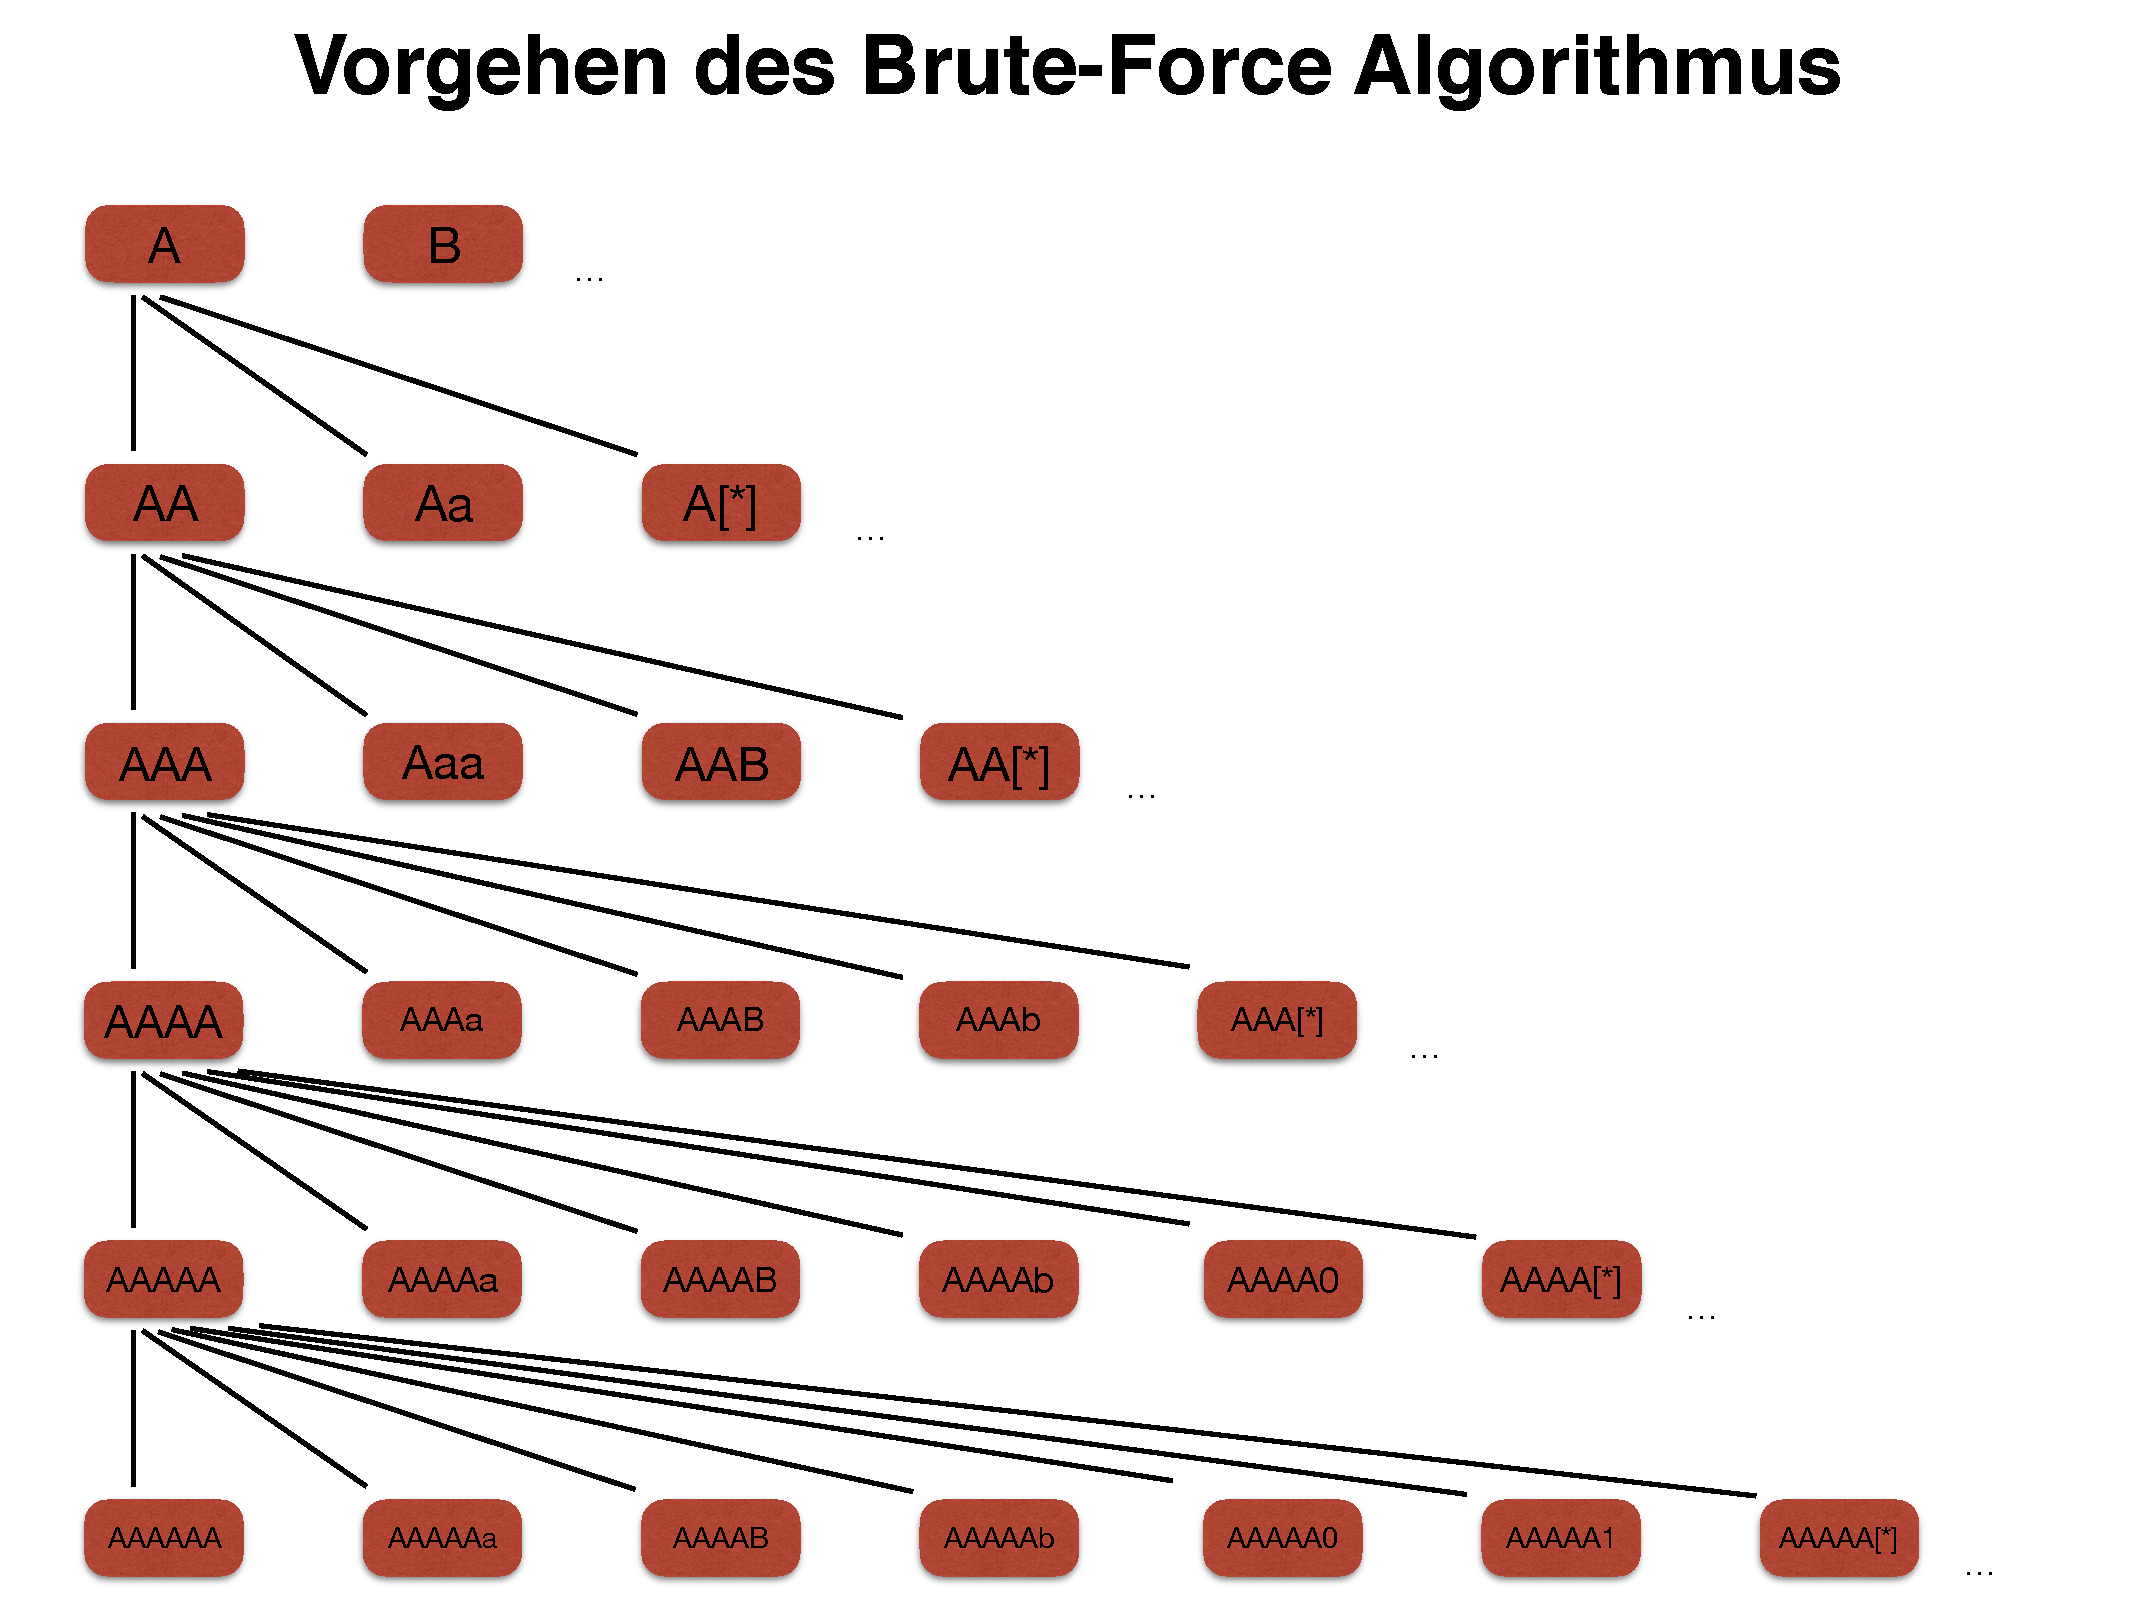
\includegraphics[natwidth=1200pt, natheight=349pt, width=1.0\textwidth]{images/SchaubildAlgorithmBreitensuche.pdf}
	\caption{Darstellung der Suchstrategie, die der Brute-Force Algorithmus zum Ermitteln des Passwortes benutzt.}
	\label{fig:showcase}
\end{figure}

%Hier Breitensuche einfügen



